%% -*- coding:utf-8 -*-
\chapter{Objects and morphisms}

\section{Equality}

The important question is how can we decide whenever an
object/morphism is equal to another object/morphism? The trivial
answer is possible if an \mynameref{def:object} is a
\mynameref{def:set}. In the case we can say that 2 objects are equal
if they contain the equivalent collection of elements. Unfortunately
we cannot do the same trick for categorical \mynameref{def:object}s as
soon as they don't have any internal 
structure but can use a \mynameref{def:categorical_approach} (see 
\mynameref{rem:set_vs_category}): if we cannot use ``microscope'' lets
use ``telescope'' and define the equality of objects and morphisms of
a category $\cat{C}$ in the terms of whole $\cathom{C}$.

\begin{definition}[Objects equality]
\label{def:object_equality}
Two \mynameref{def:object}s $a$ and $b$ in \mynameref{def:category}
$\cat{C}$ are equal if there exists an unique
\mynameref{def:isomorphism} $a \cong_f b$. This also means that
also exist unique isomorphism $b \cong_g a$. These two
\mynameref{def:morphism}s ($f$ and $g$) are related each other via 
the following equations: $f \circ g = \idm{a}$ and $g \circ f
= \idm{b}$. 
\end{definition}

Unlike \mynameref{def:function}s between \mynameref{def:set}s we don't
have any additional info 
\footnote{
for instance info about sets internals. i.e. which elements of the sets
are connected by the considered functions
}
about \mynameref{def:morphism}s except
category theory axioms which the morphisms satisfy 
\cite{bib:stackexchange:morphism:equality}. This leads us to the
following definition of morphims equality:
\begin{definition}[Morphisms equality]
\label{def:morphism_equality}
Two \mynameref{def:morphism}s $f$ and $g$ in \mynameref{def:category}
$\cat{C}$ are equal if the equality can be derived from the base axioms: 
\begin{itemize}
\item \mynameref{axm:composition}
\item \mynameref{axm:associativity}
\item \mynameref{def:id}: \eqref{eq:leftid}, \eqref{eq:rightid}
\end{itemize}
or \mynameref{def:commutative_diagram}s which postulate the equality.
\end{definition}
As an example lets proof the following theorem
\begin{theorem}[Identity is unique]
\label{thm:identity_unique}
The \mynameref{def:id} is unique.
\begin{proof}
Consider an \mynameref{def:object} $a$ and it's \mynameref{def:id} 
$\idm{a}$. Let $\exists f: a \to a$ such that $f$ is also
identity. In the case \eqref{eq:leftid} for $f$ as identity gives
\[
f \circ \idm{a} = \idm{a}.
\]
From other side \eqref{eq:rightid} for $\idm{a}$ satisfied
\[
f \circ \idm{a} = f
\]
i.e.
\[
f = f \circ \idm{a} = \idm{a}
\] 
or
$f = \idm{a}$.
\end{proof}
\end{theorem}

\section{Initial and terminal objects}
\begin{definition}[Initial object]
\label{def:initial_object}
Let $\cat{C}$ is a \mynameref{def:category}, the
\mynameref{def:object} $i \in \catob{C}$ is called
\textit{initial object} if $\forall x \in \catob{C}
\exists! f_x: i \to x \in \cathom{C}$.
\end{definition}

\begin{example}[Initial object][\textbf{Set}]
\label{ex:set_initial_object}
Note that there is only one function from empty set to any other sets
\cite{bib:proofwiki:Empty_Mapping_is_Unique} that makes the empty set
as the \mynameref{def:initial_object} in \mynameref{def:setcategory}. 
\end{example}

\begin{definition}[Terminal object]
\label{def:terminal_object}
Let $\cat{C}$ is a \mynameref{def:category}, the
\mynameref{def:object} $t \in \catob{C}$ is called
\textit{terminal object} if $\forall x \in \catob{C}
\exists! g_x: x \to t \in \cathom{C}$.
\end{definition}

\begin{example}[Terminal object][\textbf{Set}]
\label{ex:set_terminal_object}
\mynameref{def:terminal_object} in \mynameref{def:setcategory} is a set
with one element i.e \mynameref{def:singleton_set}. 
\end{example}

As you can see the initial and terminal objects are opposite each
other. I.e. if $i$ is an \mynameref{def:initial_object} in $\cat{C}$
then it will be \mynameref{def:terminal_object} in
the \mynameref{def:op_category} $\cat{C^{op}}$.

\begin{theorem}[Initial object is unique]
\label{thm:initial_object_unique}
Let $\cat{C}$ is a category and $i, i' \in \catob{C}$ two
\mynameref{def:initial_object}s then there exists an unique
\mynameref{def:isomorphism} $u: i \to i'$ (see
\mynameref{def:object_equality}) 
\begin{proof}
Consider the following \mynameref{def:commutative_diagram} (see
\cref{fig:initial_object_unique}). As soon as $i$ initial object
$\exists! \, u: i \to i'$. From other side $i'$ is also initial object
and therefore $\exists! \, u^{-1}: i' \to i$. Combining them together
via composition we can get $u^{-1} \circ u: i \to i$ and $u \circ
u^{-1}: i' \to i'$. From the fact that $i$ is initial object one can
get that there exists
only one morphism $\idm{i}: i \to i$. The same is the truth for $i'$.
Therefore $u^{-1} \circ u = \idm{i}$ and $u \circ u^{-1} = \idm{i'}$.
These complete the commutative diagram build and finishes the proof. 
\begin{figure}
  \centering
  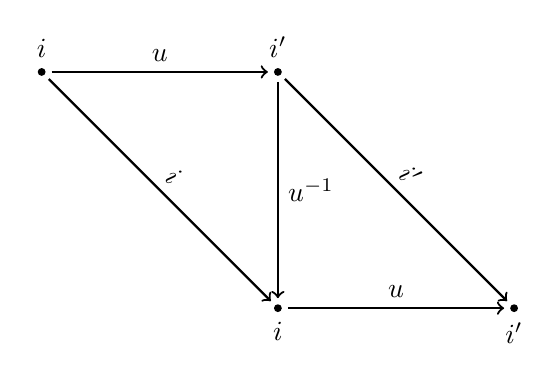
\begin{tikzpicture}[ele/.style={fill=black,circle,minimum
        width=.8pt,inner sep=1pt},every fit/.style={ellipse,draw,inner
        sep=-2pt}]

    % the texts
    
    \node[ele,label=above:$i$] (i1) at (0,3) {};    
    \node[ele,label=above:$i'$] (i2) at (3,3) {};    
    \node[ele,label=below:$i$] (i12) at (3,0) {};
    \node[ele,label=below:$i'$] (i22) at (6,0) {};

    \draw[->,thick,shorten <=2pt,shorten >=2pt] (i1) to
    node[sloped,above]{$u$} (i2);
    \draw[->,thick,shorten <=2pt,shorten >=2] (i12) to
    node[sloped,above]{$u$} (i22); 
    \draw[->,thick,shorten <=2pt,shorten >=2] (i1) to
    node[sloped,above]{$\idm{i}$} (i12); 
    \draw[->,thick,shorten <=2pt,shorten >=2] (i2) to
    node[sloped,above]{$\idm{i'}$} (i22); 
    \draw[->,thick,shorten <=2pt,shorten >=2] (i2) to
    node[right]{$u^{-1}$} (i12); 
  \end{tikzpicture}
  \caption{Commutative diagram for initial object uniqueness  proof}
  \label{fig:initial_object_unique}
\end{figure}
\end{proof}
\end{theorem}

\begin{theorem}[Terminal object is unique]
\label{thm:terminal_object_unique}
Let $\cat{C}$ is a category and $t, t' \in \catob{C}$ two
\mynameref{def:terminal_object}s then there exists an unique
\mynameref{def:isomorphism} $v: t' \to t$ (see
\mynameref{def:object_equality}) 
\begin{proof}
Just got to the \mynameref{def:op_category} and revert arrows in
\cref{fig:initial_object_unique}. The result shown on
\cref{fig:terminal_object_unique} and it proofs the theorem statement.
\begin{figure}
  \centering
  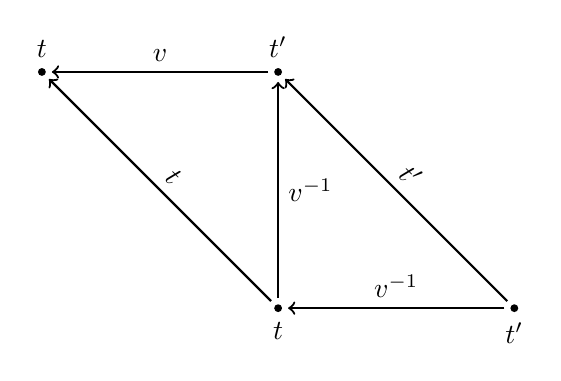
\begin{tikzpicture}[ele/.style={fill=black,circle,minimum
        width=.8pt,inner sep=1pt},every fit/.style={ellipse,draw,inner
        sep=-2pt}]

    % the texts
    
    \node[ele,label=above:$t$] (t1) at (0,3) {};    
    \node[ele,label=above:$t'$] (t2) at (3,3) {};    
    \node[ele,label=below:$t$] (t12) at (3,0) {};
    \node[ele,label=below:$t'$] (t22) at (6,0) {};

    \draw[->,thick,shorten <=2pt,shorten >=2pt] (t2) to
    node[sloped,above]{$v$} (t1);
    \draw[->,thick,shorten <=2pt,shorten >=2] (t22) to
    node[sloped,above]{$v^{-1}$} (t12); 
    \draw[->,thick,shorten <=2pt,shorten >=2] (t12) to
    node[sloped,above]{$\idm{t}$} (t1); 
    \draw[->,thick,shorten <=2pt,shorten >=2] (t22) to
    node[sloped,above]{$\idm{t'}$} (t2); 
    \draw[->,thick,shorten <=2pt,shorten >=2] (t12) to
    node[right]{$v^{-1}$} (t2); 
  \end{tikzpicture}
  \caption{Commutative diagram for terminal object uniqueness proof}
  \label{fig:terminal_object_unique}
\end{figure}
\end{proof}
\end{theorem}

\begin{example}[Toy example]
In our toy example \cref{fig:pl_example} the type String is
\mynameref{def:initial_object} and type Bool is the
\mynameref{def:terminal_object}.
\end{example}

\section{Product and sum}
The pair of 2 objects is defined via the universal property in
the following way:
\begin{definition}[Product]
\label{def:product}
Let we have a category $\cat{C}$ and $c_1, c_2 \in \catob{C}$ -two
\mynameref{def:object}s then the product of the objects $c_1, c_2$ is
another object in $\cat{C}$ $c = c_1 \times c_2$ with 2
\mynameref{def:morphism}s $\pi_1, \pi_2$ such that $c_1 = \pi_1(c),
c_2 = \pi(c_2)$ and the  
following universal property is satisfied: $\forall c' \in \catob{C}$
and morphisms $\pi'_1: c' \to c_1, \pi'_2: c' \to c_2$, exists unique
morphism $h$ such that the following diagram (see \cref{fig:product})
commutes, i.e. $\pi'_1 = \pi_1 \circ h, \pi'_2 = \pi_2 \circ h$.
\begin{figure}
  \centering
  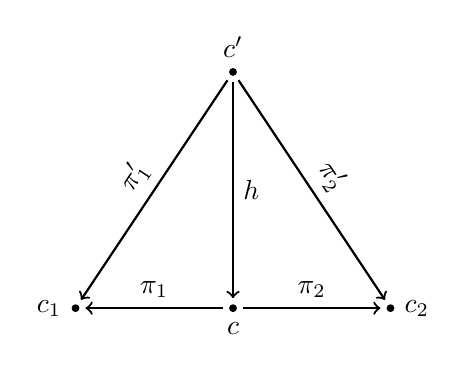
\begin{tikzpicture}[ele/.style={fill=black,circle,minimum
        width=.8pt,inner sep=1pt},every fit/.style={ellipse,draw,inner
        sep=-2pt}]

    % the texts
    
    \node[ele,label=left:$c_1$] (a) at (0,0) {};    
    \node[ele,label=right:$c_2$] (b) at (4,0) {};    
    \node[ele,label=below:$c$] (c) at (2,0) {};
    \node[ele,label=above:$c'$] (c') at (2,3) {};

    \draw[->,thick,shorten <=2pt,shorten >=2pt] (c) to
    node[sloped,above]{$\pi_1$} (a);
    \draw[->,thick,shorten <=2pt,shorten >=2] (c) to
    node[sloped,above]{$\pi_2$} (b); 
    \draw[->,thick,shorten <=2pt,shorten >=2] (c') to
    node[sloped,above]{$\pi'_1$} (a); 
    \draw[->,thick,shorten <=2pt,shorten >=2] (c') to
    node[sloped,above]{$\pi'_2$} (b); 
    \draw[->,thick,shorten <=2pt,shorten >=2] (c') to
    node[right]{$h$} (c); 
  \end{tikzpicture}
  \caption{Product $c = c_1 \times c_2$. $\forall c, \exists! h \in
    \cathom{C}: \pi'_1 = \pi_1 \circ h, \pi'_2 = \pi_2 \circ h$.}
  \label{fig:product}
\end{figure}
In other words $h$ factorizes $\pi'_{1,2}$.
\end{definition}

\begin{example}[Product][\textbf{Set}]
\label{ex:set_product}
The \mynameref{def:product} of two sets $A$ and $B$ in
\mynameref{def:setcategory} is defined 
as a \mynameref{def:cartesian_product}: $A \times B = \{(a,b)| a \in A, b \in B\}$. 
\end{example}

If we invert arrows in \mynameref{def:product} we will got another
object definition that is called sum

\begin{definition}[Sum]
\label{def:sum}
Let we have a category $\cat{C}$ and $c_1, c_2 \in \catob{C}$ -two
\mynameref{def:object}s then the sum of the objects $c_1, c_2$ is
another object in $\cat{C}$ $c = c_1 \oplus c_2$ with 2
\mynameref{def:morphism}s $i_1, i_2$ such that $c = i_1(c_1), c = i_2
(c_2)$ and the 
following universal property is satisfied: $\forall c' \in \catob{C}$
and morphisms $i'_1: c_1 \to c', i'_2: c_2 \to c'$, exists unique
morphism $h$ such that the following diagram (see \cref{fig:sum})
commutes, i.e. $i'_1 = h \circ i_1, i'_2 = h \circ i_2$.
\begin{figure}
  \centering
  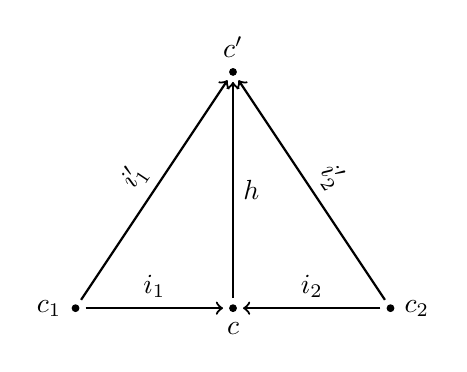
\begin{tikzpicture}[ele/.style={fill=black,circle,minimum
        width=.8pt,inner sep=1pt},every fit/.style={ellipse,draw,inner
        sep=-2pt}]

    % the texts
    
    \node[ele,label=left:$c_1$] (a) at (0,0) {};    
    \node[ele,label=right:$c_2$] (b) at (4,0) {};    
    \node[ele,label=below:$c$] (c) at (2,0) {};
    \node[ele,label=above:$c'$] (c') at (2,3) {};

    \draw[->,thick,shorten <=2pt,shorten >=2pt] (a) to
    node[sloped,above]{$i_1$} (c);
    \draw[->,thick,shorten <=2pt,shorten >=2] (b) to
    node[sloped,above]{$i_2$} (c); 
    \draw[->,thick,shorten <=2pt,shorten >=2] (a) to
    node[sloped,above]{$i'_1$} (c'); 
    \draw[->,thick,shorten <=2pt,shorten >=2] (b) to
    node[sloped,above]{$i'_2$} (c'); 
    \draw[->,thick,shorten <=2pt,shorten >=2] (c) to
    node[right]{$h$} (c'); 
  \end{tikzpicture}
  \caption{Sum $c = c_1 \oplus c_2$. $\forall c, \exists! h \in
    \cathom{C}: i'_1 = h \circ i_1, i'_2 = h \circ i_2 $.}
  \label{fig:sum}
\end{figure}
In other words $h$ factorizes $i'_{1,2}$.
\end{definition}

\begin{definition}[Disjoint union]
  \label{def:disjoint_union}
  Let $\{A_i: i \in I\}$ be a family of sets 
  indexed by $I$. The 
  \textit{disjoint union} \cite{wiki:disjointunion} of this family is
  the set 
  \[
  \sqcup_{i \in I} A_i = \cup_{i \in I}\left\{
  \left(x, i\right): x \in A_i
  \right\}.
  \]
  The elements of the disjoint union are ordered pairs $(x, i)$. Here $i$
  serves as an auxiliary index that indicates which $A_i$ the element $x$
  came from.
\end{definition}

\begin{example}[Sum][\textbf{Set}]
  \label{ex:set_sum}
  The \mynameref{def:sum} of two sets $A$ and $B$ in
  \mynameref{def:setcategory} is defined as
  \mynameref{def:disjoint_union}.  
\end{example}

The \mynameref{def:product} of objects will provide also a definition
for product of morphisms
\begin{definition}[Product of morphisms]
\label{def:product_of_morphisms}
Let $\cat{C}$ is a category and $a,a' \in \catob{C}$ and 
$b, b' \in \catob{C}$ are 2 pairs of \mynameref{def:object}s that admit
\cref{def:product}. Consider 2 morphisms that connects the objects: 
$f: a \to b, f': a' \to b'$ then we can create a new unique morphism that
connects the products: $f \times f': a \times a' \to b \times b'$ and
makes the diagram commute (see \cref{fig:product_of_morphisms}). 

\begin{figure}
  \centering
  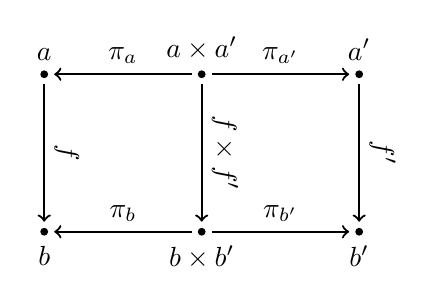
\begin{tikzpicture}[ele/.style={fill=black,circle,minimum
        width=.8pt,inner sep=1pt},every fit/.style={ellipse,draw,inner
        sep=-2pt}]

    % the texts
    
    \node[ele,label=above:$a$] (a) at (0,2) {};    
    \node[ele,label=above:$a \times a'$] (aa') at (2,2) {};    
    \node[ele,label=above:$a'$] (a') at (4,2) {};    
    \node[ele,label=below:$b$] (b) at (0,0) {};    
    \node[ele,label=below:$b \times b'$] (bb') at (2,0) {};    
    \node[ele,label=below:$b'$] (b') at (4,0) {};    

    \draw[->,thick,shorten <=2pt,shorten >=2pt] (a) to
    node[sloped,above]{$f$} (b);
    \draw[->,thick,shorten <=2pt,shorten >=2pt] (a') to
    node[sloped,above]{$f'$} (b');
    \draw[->,thick,shorten <=2pt,shorten >=2pt] (aa') to
    node[sloped,above]{$f \times f'$} (bb');


    \draw[->,thick,shorten <=2pt,shorten >=2pt] (aa') to
    node[sloped,above]{$\pi_a$} (a);
    \draw[->,thick,shorten <=2pt,shorten >=2] (aa') to
    node[sloped,above]{$\pi_{a'}$} (a'); 
    \draw[->,thick,shorten <=2pt,shorten >=2pt] (bb') to
    node[sloped,above]{$\pi_b$} (b);
    \draw[->,thick,shorten <=2pt,shorten >=2] (bb') to
    node[sloped,above]{$\pi_{b'}$} (b'); 
  \end{tikzpicture}
  \caption{Product of morphisms.}
  \label{fig:product_of_morphisms}
\end{figure}
\end{definition} 

\section{Category as a monoid}
Consider the following definition from abstract algebra
\begin{definition}[Monoid]
  \label{def:monoid}
  The set of elements $M$ with defined binary operation $\circ$ we will call
  as a monoid if the following conditions are satisfied.
  \begin{enumerate}
  \item Closure: $\forall a, b \in M$: $a \circ b \in M$
  \item Associativity: $\forall a, b, c \in M$:
    $a \circ \left( b \circ c \right) =
    \left( a \circ b \right) \circ c$
  \item Identity element: $\exists e \in M$ such that
    $\forall a \in M$: $e \circ a = a \circ e = a$
  \end{enumerate}
\end{definition}

We can consider 2 \mynameref{def:monoid}s. The first one has
\mynameref{def:product} as the binary operation and
\mynameref{def:terminal_object} as the identity element. As result we
just got an analog of multiplication in the category theory. This is why
the terminal object is often denoted as $\mathbf{1}$ and the operation
is called as the product. 

Another one is additional \mynameref{def:monoid} that has
\mynameref{def:initial_object} as the identity element and the
\mynameref{def:sum} as the binary operation. The initial object in
that case  is often denoted as $\mathbf{0}$. I.e. we can see a direct
connection with addition in algebra.

If we do such consideration then we can make a step forward and look
at the distributive law that sum and multiplication satisfy.
\begin{definition}[Distributive category]
\label{def:distributive_category}
A category $\cat{C}$ is \textit{distributive} if 
\cite{wiki:distributive_category}
it has finite
\mynameref{def:product}s and \mynameref{def:sum}s such that 
$\forall a,b,c \in \catob{C}$:
\[
a \times b \oplus a \times c \cong a \times ( b \oplus c )
\]
and 
\[
a \times 0 \cong 0
\]
where $\mathbf{0}$ is the \mynameref{def:initial_object}.
\end{definition} 

\begin{example}[Distributive category]
\label{ex:distributive_category}
\mynameref{def:setcategory} is an example 
\cite{wiki:distributive_category}
of \mynameref{def:distributive_category}

From other hand not all categories which have both product and sum are
distributive. One of such example is a category of all groups
\cite{wiki:distributive_category} 
$\cat{Grp}$ where groups are considered as objects and group
homomorphisms as morphisms. 
\end{example}

\section{Exponential}
We are going to talk about functions (aka morphisms) as
\mynameref{def:object}s. 

\begin{example}[Hom set]
\label{ex:homset}
Consider 2 sets $A$ and $B$ the set of functions between the 2 sets
form a new set that is called as \textit{Hom-set} and denoted as $A
\to B$. Thus if $A,B \in \catob{Set}$ then the Hom-set will also $A
\to B \in \catob{Set}$. 
\end{example}

The construction of \mynameref{ex:homset} is applied to
\mynameref{def:setcategory} but not to an arbitrary category because
the Hom-set is a set and therefore the object in the \textbf{Set}
category. I.e. if $\cat{C}$ is a category and $a, b \in \catob{C}$
then the Hom-set $a \to b \in \catob{Set}$ but we now want to
construct something like to the Home-set but that is an object in
$\cat{C}$. This will be called as the function object. We will use the
universal construction for the object definition.

\begin{definition}[Exponential]
\label{def:exponential}
\begin{figure}
  \centering
  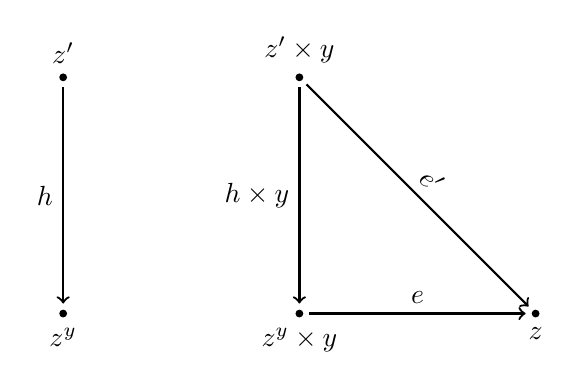
\begin{tikzpicture}[ele/.style={fill=black,circle,minimum
        width=.8pt,inner sep=1pt},every fit/.style={ellipse,draw,inner
        sep=-2pt}]

    % the texts
    
    \node[ele,label=above:$z'$] (z1) at (0,3) {};    
    \node[ele,label=below:$z^y$] (zy) at (0,0) {};    
    \node[ele,label=above:$z' \times y$] (z1y) at (3,3) {};
    \node[ele,label=below:$z^y \times y$] (zyy) at (3,0) {};
    \node[ele,label=below:$z$] (z) at (6,0) {};

    \draw[->,thick,shorten <=2pt,shorten >=2pt] (z1) to
    node[left]{$h$} (zy);
    \draw[->,thick,shorten <=2pt,shorten >=2] (z1y) to
    node[left]{$h \times \idm{y}$} (zyy); 
    \draw[->,thick,shorten <=2pt,shorten >=2] (z1y) to
    node[sloped,above]{$e'$} (z); 
    \draw[->,thick,shorten <=2pt,shorten >=2] (zyy) to
    node[sloped,above]{$e$} (z); 
  \end{tikzpicture}
  \caption{Exponential object}
  \label{fig:exponential}
\end{figure}
Let $\cat{C}$ is a category and $z, y \in \catob{C}$. We also assume
that $\cat{C}$ allows all \mynameref{def:product}s with $y$, i.e.
$\forall z' \in \catob{C}, \exists z' \times y$. An object $z^y$
together with a \mynameref{def:morphism} $e: z^y \times y \to z$ is 
an \textit{exponential object} if $\forall e' \in \cathom{C}$ and
$\forall z' \in \catob{C}$ exists an
unique morphism $h: z' \to z$ such that the
\mynameref{def:commutative_diagram} shown in \cref{fig:exponential}
commutes:
\[
e' = e \circ \left(h \times \idm{y} \right)
\]
\end{definition}

\begin{example}[Exponential][\textbf{Set}]
\label{ex:exponential_set}
Lets look at the \mynameref{def:exponential} in $\cat{Set}$. We want
to show that the object corresponds to the function. Really if we want
to define a function $f: X \to Y$ then we should look at the
\mynameref{ex:homset} $F = X \to Y$. $f \in F$ - is an element of the
Hom-set. For the function application we have to take the argument $x
\in X$ and the function we want to apply $f \in F$. Then we construct
the pair $(f,x) \in F \times X$. For the function application we have
to call a \mynameref{def:morphism} $e: F \times X \to Z$.
\footnote{$e$ from the word ``eval''}
I.e. the
application $e(f, x)$ gives us $e(f, x) = y \in Y$ - the function
value. 
\end{example}

\begin{definition}[Cartesian closed category]
\label{def:cartesian_closed_category}
If a category $\cat{C}$ satisfies the following conditions then it is
called \textit{Cartesian closed category}
\begin{enumerate}
\item It has \mynameref{def:terminal_object}
\item $\forall a,b \in \catob{C}$ exists \mynameref{def:product} $a
  \times b \in \catob{C}$.
\item $\forall a,b \in \catob{C}$ exists \mynameref{def:exponential}
  $a^b \in \catob{C}$
\end{enumerate}
\end{definition}

\begin{theorem}[Cartesian closed category]
\label{thm:ccc}
If $\cat{C}$ is a \mynameref{def:cartesian_closed_category} with
finite \mynameref{def:sum} then it is a
\mynameref{def:distributive_category}.
\begin{proof}
TBD
\end{proof}
\end{theorem}

\section{Type algebra and Curry-Howard-Lambek correspondence}
\label{sec:curry_howard_lambek}
There is an interesting correspondence between computer programs and
mathematical proofs. First of all consider a category of proofs
\subsection{\textbf{Proof} category}
\begin{definition}[Proposition]
\label{def:proposition}
\textit{Proposition} is a statement that either true or false.
\end{definition}

There are 2 main propositions
\begin{definition}[True]
\label{def:true}
A true statement is one that is correct, either in all cases or at
least in the sample case \cite{bib:studycom:truefalse}. 
\end{definition}
and
\begin{definition}[False]
\label{def:false}
A false statement is one that is not correct \cite{bib:studycom:truefalse}. 
\end{definition}


\begin{example}[Proposition]
\label{ex:proposition}
There is an example of correct (true) proposition
\[
\forall n \in \mathbb{R}: n^2 \ge 0
\]

There is an example of incorrect (false) proposition
\[
\forall n \in \mathbb{C}: n^2 \ge 0,
\]
for instance $i \in \mathbb{C}$ gives $i^2 = -1$.

\end{example}

\begin{definition}[Implication]
\label{def:implication} \textit{An implication} is a
\mynameref{def:proposition} of the form $P \implies Q$ i.e. if $P$
then $Q$ \cite{bib:whatisaproof}.
\end{definition}

The main logical deduction rule is the following
\begin{definition}[Modus ponens]
\label{def:modusponens}
If $P$ is true and $P \implies Q$ is true then $Q$ is also true. The
rule is often written as \cite{bib:whatisaproof}
\[
\frac{
\begin{array}{c}
P \\
P \implies Q
\end{array}
}{Q}
\]
where if statements above the line are true then the statement below
the line is also true.
\end{definition}

\begin{definition}[Proof]
\label{def:proof}
\textit{Proof} is a verification \cite{bib:whatisaproof} of a
\mynameref{def:proposition} by a chain of logical deduction from a
base set of axioms.
\end{definition}

Propositions can be combined into new propositions via the following
logical operations
\begin{definition}[Conjunction]
\label{def:conjunction}
Conjunction or logical AND is the operation with following rules
  \begin{table}[H]
    \centering
    \caption{Conjunction}
    \label{tab:conjunction}
      \begin{tabular}{|l|l|l|}
        \hline
        $a$ & $b$ & $a \land b$ \\ \hline
        True & True & True \\ \hline
        True & False & False \\ \hline
        False & True & False \\ \hline
        False & False & False \\ \hline
      \end{tabular}
  \end{table}
\end{definition}
\begin{definition}[Disjunction]
\label{def:disjunction}
Conjunction or logical OR is the operation with following rules
  \begin{table}[H]
    \centering
    \caption{Disjunction}
    \label{tab:disjunction}
      \begin{tabular}{|l|l|l|}
        \hline
        $a$ & $b$ & $a \lor b$ \\ \hline
        True & True & True \\ \hline
        True & False & True \\ \hline
        False & True & True \\ \hline
        False & False & False \\ \hline
      \end{tabular}
  \end{table}
\end{definition}

Operations in Boolean logic follow the distributive low:
\begin{equation}
a \land ( b \lor c) = (a \land b) \lor (a \land c) 
\nonumber
\end{equation}
i.e. the operation $\land$ corresponds to multiplication and $\lor$ to
sum. Therefore the $\cat{Proof}$ can be considered as a
\mynameref{def:distributive_category}. 

\begin{definition}[\textbf{Proof} category]
\label{def:proof_category}
The $\cat{Proof}$ category is a category where \mynameref{def:proposition}s are
\mynameref{def:object}s and \mynameref{def:proof}s are
\mynameref{def:morphism}s. I.e. proofs are used as connectors between
different propositions.
\end{definition}

Consider different objects and constructions of the proof (logic)
theory from the categorical point of view
\begin{example}[Initial object][\textbf{Proof}]
\label{ex:proof_initial_object}
The \textit{false} statement can be considered as the initial object
because for any other statement exists only one proof from the false
statement to that one.
\end{example}

\begin{example}[Terminal object][\textbf{Proof}]
\label{ex:proof_terminal_object}
The \textit{true} statement can be considered as the terminal object
\end{example}

\begin{example}[Product][\textbf{Proof}]
\label{ex:proof_product}
\mynameref{def:conjunction} can be considered as
\mynameref{def:product} in \mynameref{def:proof_category}.
\end{example}

\begin{example}[Sum][\textbf{Proof}]
\label{ex:proof_sum}
\mynameref{def:disjunction} can be considered as
\mynameref{def:sum} in \mynameref{def:proof_category}.
\end{example}

Thus we can declare the following correspondence (see
\cref{tab:curry_howard_lambek}) between logic 
proofs and \mynameref{def:cartesian_closed_category} and therefore
also between programming languages.
\begin{table}[H]
  \centering
  \caption{Relation between logic proofs and programming languages}
  \label{tab:curry_howard_lambek}
  \begin{adjustbox}{width=1\textwidth}
    \small
    \begin{tabular}{l|l|l}
      \toprule
      \mynameref{def:proof_category} & Programming language & 
      \mynameref{def:cartesian_closed_category}\\
      \midrule
      \mynameref{def:proposition}/\mynameref{def:implication} & Type &
      \mynameref{def:object} \\ 
      \mynameref{def:proof} & Function type & \mynameref{def:exponential} \\
      \mynameref{def:conjunction} & Product type & \mynameref{def:product} \\
      \mynameref{def:disjunction} & Sum type & \mynameref{def:sum} \\
      \mynameref{def:true} & unit type & \mynameref{def:terminal_object} \\
      \mynameref{def:false} & botom type & \mynameref{def:initial_object} \\
      \bottomrule
    \end{tabular}
  \end{adjustbox}
\end{table}

\subsection{\textbf{Hask} category}
\begin{example}[Initial object][\textbf{Hask}]
If we avoid lazy evaluations in Haskell (see
\mynameref{rem:hask_lazy_eval}) then we can found several types
as candidates for initial and terminal object in Haskell. 
\label{ex:hask_initial_object}
\mynameref{def:initial_object} in \mynameref{def:haskcategory} is a
type without values 
\begin{minted}{haskell}
data Void
\end{minted}
i.e. you cannot construct a object of the type.

There is only one function from the initial object:
\begin{minted}{haskell}
absurd :: Void -> a
\end{minted}
The function is called absurd because it does absurd action. Nobody
can proof that it does not exist. For the existence proof the
following absurd argument can be used: ``Just provide me an object type
\textbf{Void} and I will provide you the result of
evaluation''.  

There is no function in opposite direction because it would had been
used for the \textbf{Void} object creation. 
\end{example}

\begin{example}[Terminal object][\textbf{Hask}]
\label{ex:hask_terminal_object}
Terminal object (unit) in \mynameref{def:haskcategory} keeps only one element
\begin{minted}{haskell}
data () = ()
\end{minted}
i.e. you can create only one element of the type. You can use the
following function for the creation:
\begin{minted}{haskell}
unit :: a -> ()
unit _ = ()
\end{minted}
\end{example}

\begin{example}[Product][\textbf{Hask}]
\label{ex:hask_product}
The \mynameref{def:product} in \mynameref{def:haskcategory} keeps a
pair and the constructor defined as follows
\begin{minted}{haskell}
(,) :: a -> b -> (a, b)
(,) x y = (x, y)
\end{minted}
There are 2 projectors: 
\begin{minted}{haskell}
fst :: (a, b) -> a
fst (x, _) = x
snd :: (a, b) -> b
snd (_, y) = y
\end{minted}
\end{example}

\begin{example}[Sum][\textbf{Hask}]
\label{ex:hask_sum}
The \mynameref{def:sum} in \mynameref{def:haskcategory} defined as
follows 
\begin{minted}{haskell}
data Either a b = Left a | Right b
\end{minted}

The typical usage is via pattern matching for instance 
\begin{minted}{haskell}
factor :: (a -> c) -> (b -> c) -> Either a b -> c
factor f _ (Left x) = f x
factor _ g (Right y) = g y
\end{minted}
\end{example}

\begin{example}[Distributive category][\textbf{Hask}]
As soon as $\cat{Hask}$ is a \mynameref{def:cartesian_closed_category}
then by \cref{thm:ccc} it is a \mynameref{def:distributive_category}
i.e. one can conclude that
\begin{minted}{haskell}
(a,Either b c)
\end{minted}
is the same to
\begin{minted}{haskell}
Either (a, b) (a, c)
\end{minted}
\end{example}

\begin{example}[Exponential][\textbf{Hask}]
\label{ex:exponential_hask}
It's not surprisingly that the \mynameref{def:exponential} in
$\cat{Hask}$ is a function object i.e. $b^a$ can be written as  
\textbf{a -> b}.
\end{example}

\begin{example}[Type algebra]
\cref{ex:exponential_hask} gives interesting results with types
manipulations. For instance the type $a^{b+c}$ can be written as
\begin{minted}{haskell}
Either b c -> a
\end{minted}
for the function we should have both functions 
\textbf{b -> a} and \textbf{b -> c}. I.e.
the code is equivalent to the following one
\begin{minted}{haskell}
(b -> a, c -> a)
\end{minted}
These transformations correspond to the following simple algebraic
equation 
\[
a^{b+c} = a^b a^c.
\]
This is also called as \textit{type algebra}.
\end{example}

\subsection{\textbf{C++} category}
\begin{example}[Initial object][\textbf{C++}]
\label{ex:cpp_initial_object}
In C++ exists a special type that does not hold any values and as
result cannot be created: \textbf{void}.
You cannot create an object of that type i.e. you will get a compiler
error if you try.
\end{example}

\begin{example}[Terminal object][\textbf{C++}]
\label{ex:cpp_terminal_object}
C++ 17 introduced a special type that keeps only one value -
\textbf{std::monostate}:  
\begin{minted}{c++}
namespace std {
  struct monostate {};
}
\end{minted}
\end{example}

\begin{example}[Product][\textbf{C++}]
\label{ex:cpp_product}
The \mynameref{def:product} in \mynameref{def:cppcategory} keeps a
pair and the constructor defined as follows
\begin{minted}{c++}
namespace std {
  template< class A, class B > struct pair {
    A first;
    B second;
  };
}
\end{minted}

There is a simple usage example
\begin{minted}{c++}
  std::pair<int, bool> p(0, false);

  std::cout << "First projector: " << p.first << std::endl;
  std::cout << "Second projector: " << p.second << std::endl;

\end{minted}
Really any \textbf{struct} or \textbf{class} can be
considered as a product. 
\end{example}

\begin{example}[Sum][\textbf{C++}]
  \label{ex:cpp_sum}
  If we consider \mynameref{def:object}s as types then
  \mynameref{def:sum} is an object that can be either one or another
  type. The corresponding C/C++ construction that provides an ability
  to keep one of two types is \textbf{union}. 

  %% There is an \textbf{Either} implementation from
  %% \mynameref{ex:hask_sum} 
  %% \begin{minted}{c++}
  %%   template <typename A, typename B> class Either
  %%   {
  %%   public:
  %%     Either(const Either& e) : is_left_(e.is_left_){
  %%       if (is_left_){
  %%         data.l = e.data.l;      
  %%       } else {
  %%         data.r = e.data.r;      
  %%       }    
  %%     }
  %%     ~Either(){
  %%       if (is_left_){
  %%         data.l.~A();      
  %%       } else {
  %%         data.r.~B();      
  %%       }        
  %%     }      
  %%     Either(const A& l) : data(l), is_left_(true){
  %%     }
  %%     Either(const B& r) : data(r), is_left_(false){
  %%     }
  %%     const A& left() const {
  %%       if (!is_left_){
  %%         throw std::logic_error("no left");      
  %%       }    
  %%       return data.l;    
  %%     }
  %%     const B& right() const {
  %%       if (is_left_){
  %%         throw std::logic_error("no right");      
  %%       }    
  %%       return data.r;    
  %%     }
  %%   private:
  %%     union Data {
  %%       Data() {}
  %%       Data( const A& a) : l(a) {}
  %%       Data (const B& b) : r(b) {}
  %%       ~Data() {}
  %%       A l;
  %%       B r;
  %%     } data;       
  %%     bool is_left_;  
  %%   };
  %% \end{minted}
  %% The usage example:
  %% \begin{minted}{c++}
  %%   template <typename A, typename B, typename C, typename D>
  %%   auto factor(A f, B g, const Either<C, D>& either) {
  %%     try {
  %%       return f(either.left());               
  %%     }
  %%     catch(...) {
  %%       return g(either.right());                              
  %%     }
  %%   };
    
  %%   auto stringLength = [](std::string s) {
  %%     return static_cast<int>(s.size()); };
  %%   auto id = [](auto x) { return x; };
          
  %%   Either<std::string, int> str = std::string("abc");
  %%   std::cout << "String length:" <<
  %%   factor<>(stringLength, id, str) << std::endl;
  %%   Either<std::string, int> i = 4;
  %%   std::cout << "id(int):" <<
  %%   factor<>(stringLength, id, i) << std::endl;
  %% \end{minted}

  C++17 suggests \textbf{std:variant} as a safe replacement
  for \textbf{union}. The example of the \textbf{factor}
  function is below
  \begin{minted}{c++}
    template <typename A, typename B, typename C, typename D>
    auto factor(A f, B g, const std::variant<C, D>& either) {
      try {
        return f(std::get<C>(either));               
      }
      catch(...) {
        return g(std::get<D>(either));                              
      }
    };
  \end{minted}
  The simple usage as follows:
  \begin{minted}{c++}
    std::variant<std::string, int> var = std::string("abc");
    std::cout << "String length:" <<
    factor<>(stringLength, id, var) << std::endl;
    var = 4;
    std::cout << "id(int):" <<
    factor<>(stringLength, id, var) << std::endl;    
  \end{minted}

\end{example}
TBD
\subsection{\textbf{Scala} category}
\begin{example}[Initial object][\textbf{Scala}]
\label{ex:scala_initial_object}
We used a same trick as for \mynameref{ex:hask_initial_object} in
\mynameref{def:haskcategory} and define
\mynameref{def:initial_object} in \mynameref{def:scalacategory} as a
type without values 
\begin{minted}{scala}
sealed trait Void
\end{minted}
i.e. you cannot construct a object of the type.
\end{example}

\begin{example}[Terminal object][\textbf{Scala}]
\label{ex:scala_terminal_object}
We used a same trick as for \mynameref{ex:hask_terminal_object}
in \mynameref{def:haskcategory} and define
\mynameref{def:terminal_object} in \mynameref{def:scalacategory} as a
type with only one value
\begin{minted}{scala}
abstract final class Unit extends AnyVal
\end{minted}
TBD
i.e. you can create only one element of the type.
\end{example}

TBD

\section{Quantum mechanics}
\begin{example}[Initial object][\textbf{FdHilb}]
\label{ex:quant_initial_object}
We will use a Hilber space of dimensional 0 as the
\mynameref{def:initial_object}. I.e. the set that does not have any
states in it.
\end{example}

\begin{example}[Terminal object][\textbf{FdHilb}]
  \label{ex:quant_terminal_object}
We will use a Hilber space of dimensional 1 as the
\mynameref{def:terminal_object}. I.e. the set of complex numbers
$\mathbb{C}$.   
\end{example}

\begin{example}[Product][\textbf{FdHilb}]
  \label{ex:quant_product}
  The \mynameref{def:product} in \mynameref{def:fdhilbcategory} is a
  \mynameref{def:fdhilb_direct_sum}.
\end{example}

\begin{example}[Sum][\textbf{FdHilb}]
  \label{ex:quant_sum}
  The \mynameref{def:sum} in \mynameref{def:fdhilbcategory} is a
  \mynameref{def:fdhilb_direct_sum}.
\end{example}

TBD

